\documentclass[tikz,border=10pt]{standalone}
\usepackage{amsmath,amssymb}
\usetikzlibrary{calc,arrows.meta}

\begin{document}
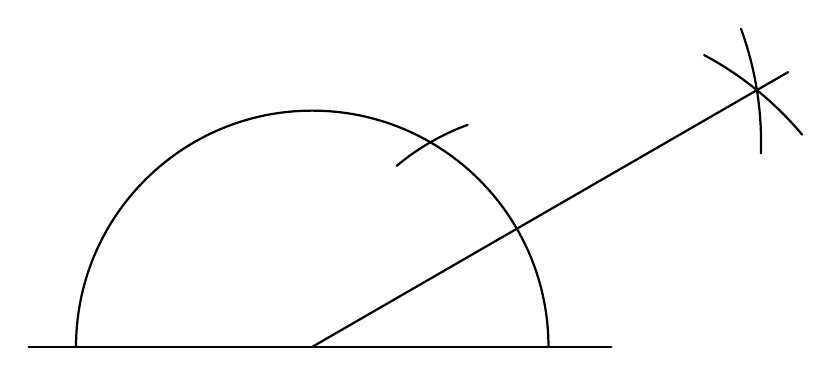
\begin{tikzpicture}[>=latex, line cap=round, line join=round]
  % Define origin and parameters
  \coordinate (O) at (0,0);
  \def\r{3.0}     % radius of main arc
  \def\R{4.2}     % radius of bisector arcs

  % Baseline
  \draw[thick] (-3.6, 0) -- (3.8, 0);

  % Main arc from O(0,0), radius r, from 0 deg to 180 deg
  \draw[thick] (\r, 0) arc (0:180:\r);

  % Intersection on baseline: P1 = (r, 0)
  \coordinate (P1) at (\r, 0);

  % 60-degree point: P2 = (r*cos 60, r*sin 60)
  \coordinate (P2) at ({\r*cos(60)}, {\r*sin(60)});

  % Arc cutting at 60 deg, centered at P1, radius r (angle 120 deg from P1)
  \draw[thick] ($(P1) + (110:\r)$) arc (110:130:\r);

  % Bisector intersection point at 30 deg
  \pgfmathsetmacro{\dmid}{\r*cos(30)}
  \pgfmathsetmacro{\h}{sqrt(\R*\R - (\r*sin(30))*(\r*sin(30)))}
  \pgfmathsetmacro{\dtotal}{\dmid + \h}
  \coordinate (X) at ({\dtotal*cos(30)}, {\dtotal*sin(30)});

  % Arc from P1 through X (radius R)
  \pgfmathsetmacro{\angOne}{atan2(\dtotal*sin(30), \dtotal*cos(30) - \r)}
  \draw[thick] ($(P1) + ({\angOne - 11}:\R)$) arc ({\angOne - 11}:{\angOne + 11}:\R);

  % Arc from P2 through X (radius R)
  \pgfmathsetmacro{\angTwo}{atan2(\dtotal*sin(30) - \r*sin(60), \dtotal*cos(30) - \r*cos(60))}
  \draw[thick] ($(P2) + ({\angTwo - 11}:\R)$) arc ({\angTwo - 11}:{\angTwo + 11}:\R);

  % Constructed 30-degree ray through X
  \draw[thick] (O) -- ({\dtotal*1.07*cos(30)}, {\dtotal*1.07*sin(30)});

\end{tikzpicture}
\end{document}
